\subsection{Sammankoppling av Androidenheter}

När telefonen på svävaren är inkopplad till ADK:n och dess applikation har startat kan
bluetoothlänken till fjärrkontrollen upprättas. För att upprätta denna länk finns det några steg som skall göras på de olika sidorna, dessa steg beskrivs nedan.

\subsubsection{Routern}

För att initiera länken trycker man på knappen Bluetooth Setup i applikationen på svävaren.
När denna knapp har trycks så har man 30 sekunder på sig att ansluta till den med fjärrkontrollen, om man inte ansluter inom den tiden så kopplas länken ner igen.
Routern måste vara synlig för andra bluetoothenheter för att den skall kunna
upptäckas av fjärrkontrollen.

\begin{figure}[htbp!]
\centering
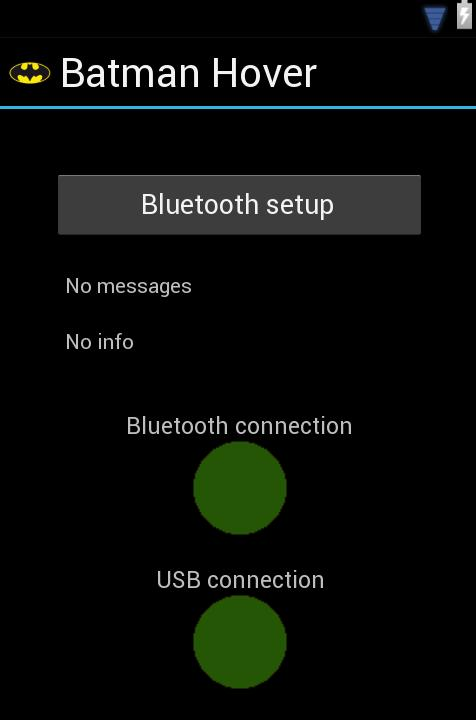
\includegraphics[width=4cm]{../../includes/figures/hoverApp.png}
\caption{Grafiskt interface för applikationen på Routern.}
\label{fig:hoverApp}
\end{figure}


\subsubsection{Fjärrkontrollen}

På fjärrkontrollen finns det tre knappar som används vid sammankopplingen, dessa är Search, Choose samt Connect. Med Search-knappen leter fjärrkontrollen efter tillgängliga bluetoothenheter i dess omgivning. När denna sökning är klar så listas alla upptäckta enheter i applikationen under Inforubriken. Med knappen Choose kan man stega genom listan med upptäckta enheter tills man kommer fram till den man vill ansluta sig till, alltså svävaren.
Search och Choose kan göras innan knappen Bluetooth Setup har tryckts i applikationen på svävaren. När man med Choose har valt svävaren på fjärrkontrollen och Bluetooth Setup har trycks på applikationen på svävaren trycks slutligen knappen Connect på fjärrkontrollen, då sammankopplas telefonerna och länken för dataöverföring är öppen.

\begin{figure}[htbp!]
\centering
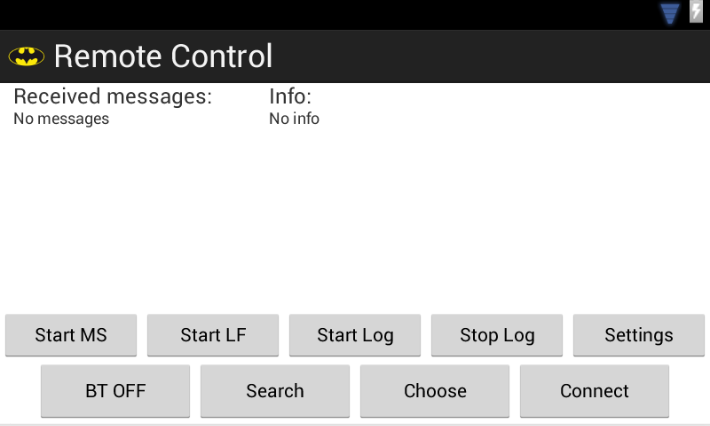
\includegraphics[width=8cm]{../../includes/figures/remoteApp.png}
\caption{Grafiskt interface för applikationen på Fjärrkontrollen.}
\label{fig:remoteApp}
\end{figure}
